\section{Kinematics}\label{sec:kinematics}
The channel proposed to be studied is 
\begin{align}
e(k)+p(p)\to e'(k') + p'(p') +\etaP(\nu) \label{eq:etaP} 
\end{align}
where $k$, $k'$, $p$, $p'$ are the four–momenta of the incident lepton, outgoing lepton,target proton and scattered proton respectively. The virtual photon in the production is defined as $q=k-k'$ with energy $v = \frac{pq}{m_p} = E - E'$. The quantity $\etaP(\nu)$ is the electro-produced meson. Production mechanisms of similar mesons have been already proposed in previous proposals~\cite{clas.proposal.eta,clas.proposal.phi} and are scheduled to run in conjunction with RunGroupA, the same run group requested for in this proposal.
The main decays studied for this proposal are:
\begin{align}
\etaP \rightarrow \gamma \gamma \to e^+e^- \gamma \label{eq:etaPconv} \\
\etaP \rightarrow \gamma \gamma^\star \to \gamma e^+e^- \label{eq:etaPDal} 
\end{align}
i.e. when a pseudoscalar meson, $P_p$($\eta'$), decays via two photons (Eq.~\ref{eq:etaPconv}) and one photon converts into an \epemT \ pair due to E.M. processes through matter, this is conventionally known as external conversions. This decay channel will be the main background contribution and is further discussed in Sec~\ref{sec:intro.conversion}. The Dalitz decay(Eq.~\ref{eq:etaPDal}), or internal conversion, is when the $P_p$($\eta'$) decays via a real photon and a virtual photon, which decays into an \epemT \ pair.
Figure~\ref{fig:piz.alldecay} illustrates the Feynman diagrams for the pseudoscalar ``two photon decay'' and  ``Dalitz decay''.
 %Table~\ref{tab:pi0}. Figure~\ref{fig:piz.alldecay} illustrates the Feynman diagrams for the ``Two photon decay'' and the ``Dalitz decay''.
 \begin{figure}[h!]\begin{center}
 		\subfloat[Feynman Diagram of $\etaP$ Two Photon Decay][]{ %Feynman diagram of $\etaP$ two photon decay
 			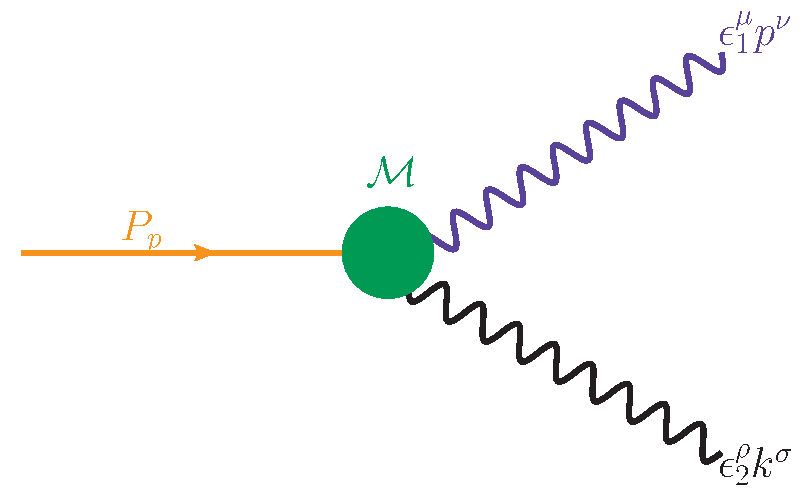
\includegraphics[width=0.4\columnwidth,height=0.75\qfigheight]{\grpath/decays/psudoscalar_gammagamma.pdf}\label{fig:piz.gamgam}
 		}
 		\quad
 		\subfloat[Feynman Diagram of $\etaP$ Dalitz Decay][]{ %Feynman diagram of $\etaP$ Dalitz decay
 			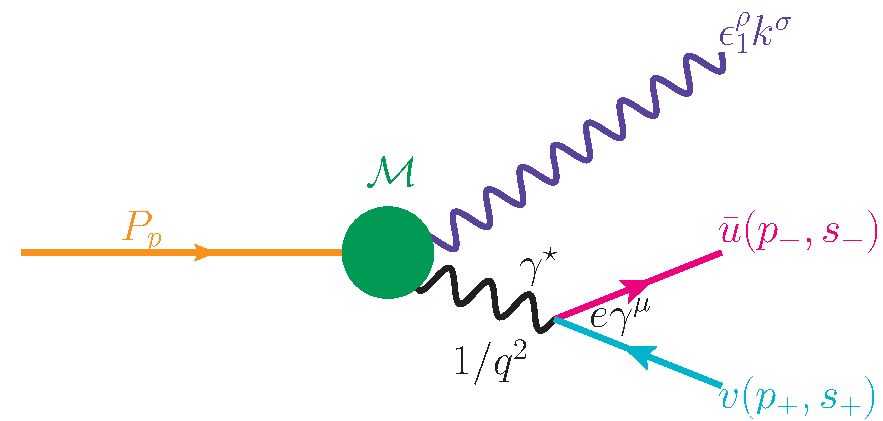
\includegraphics[width=0.45\columnwidth,height=0.75\qfigheight]{\grpath/decays/psudoscalar_dalitz.pdf}\label{fig:piz.dalitz}
 		}
 		\caption[Feynman diagram of $P_p$($\etaP$) two photon decay and Dalitz decay]{\label{fig:piz.alldecay}Feynman diagram of $P_p$($\etaP$) two photon decay~\subref{fig:piz.gamgam}, $\epsilon_1$ and $\epsilon_2$ are the polarizations, $p$ and $k$ are 4-momenta of the photons.  Feynman diagram of $P_p$($\etaP$) Dalitz decay~\subref{fig:piz.dalitz}, the variable $s_\pm$ are the spin helicities of the outgoing leptons $l^\pm$ with 4-momenta $p_{\pm}$ and $\epsilon$ is the polarization of the outgoing photon with 4-momenta $k$. In both diagrams $\mathcal{M}$ is the form factor.}
\end{center}\end{figure}
 A full derivation of the external conversion and Dalitz decay are given in the Appendix~\ref{sec:app.kinematics}.
 \FloatBarrier
  \subsection{The Dalitz Decay}
  The Dalitz decay of mesons is dependent on the spin of the meson. For pseudoscalar meson the decay rate is derived in~\ref{sec:dalitzdecay} and is expressed as:
  \begin{align}\label{eq:eegff.finalkroll_II}
  \frac{d\Gamma_{\epem \gamma}}{\Gamma_{\gamma\gamma} dq^2} = \frac{2 \alpha}{3 \pi} \frac{1}{q^2} \left( 1- \frac{q^2}{m_p^2}\right)^3 \left( 1+ \frac{2m_l^2}{q^2}\right) \left( 1- \frac{4m_l^2}{q^2}\right)^{\frac{1}{2}} 
  \end{align}
  which is the Kroll-Wada equation founded in~\cite{KrollWada,landsberg}.
   An example of QED expectation for \etaTP  \ is shown in Fig.~\ref{fig:dalitz_compare}.
  \subsection{Form Factor}
   It has been experimentally observed that the shape of the dilepton mass spectrum deviates significantly from the QED predictions, displaying a rise at larger dilepton mass. Therefore, the form factor ${M}_P(p^2,k^2=0)$ or ${M}_P(p_{1}^2,p_{2}^2)$  can be written as follows:
  \begin{align}
  {M}_P \to {M}_P' \times \left|F(q^2)\right| \ ,
  \end{align}
  where $M_P'$ is the decay constant of two photons or $\eta$ photon (as mentioned in Sec.~\ref{sec:piz.gg}), while $\left|F(q^2)\right|$ is called the transition form factor, which defines the electromagnetic space structure of the meson. According to that, the $\etaP \to e^+e^- \gamma$ the decay rate modifies as;
  \begin{align}\label{eq:eegff.final}
  \frac{d\Gamma_{\epem \gamma}}{\Gamma_{\gamma\gamma} dq^2} = \frac{2 \alpha}{3 \pi} \frac{1}{q^2} \left( 1- \frac{q^2}{m_p^2}\right)^3 \left( 1+ \frac{2m_l^2}{q^2}\right) \left( 1- \frac{4m_l^2}{q^2}\right)^{\frac{1}{2}} \left|F(q^2)\right|^2 \ ,
  \end{align}
  First observations were described with standard vector meson dominance (VMD) where the virtual photon can stem from a intermediate vector mesons. 
  The value of $\left|F(q^2)\right|$ can be directly measured by comparing QED predictions to the measured rate~\cite{landsberg}. 
  \begin{align}
  \frac{d\Gamma(A\to B+l^+l^-)}{dq^2 \Gamma(A\to B\gamma)} = \left[\frac{d\Gamma}{dq^2}\right]_{\text{QED}} \cdot \left | F(q^2) \right |^2 
  \end{align}
  or by performing a line shape analysis on the $l^{+}l^{-}$ invariant mass using assumptions on the structure of $\left|F(q^2)\right|$. One such assumption for $\left|F(q^2)\right|$ is the dipole approximation from the VMD model, which can be parametrized as:
  \begin{align}
  F(q^2) = \frac{1}{1-q^2/\Lambda^2} 
  \end{align}
   where the parameter $\Lambda$ corresponds to the mass for the effective contributing vector meson.
%  , in which 
%  \begin{align}
%  F(q^{2}) = \frac{\Lambda^2(\Lambda^2 + \gamma^2)}{(\Lambda^{2} - q^2) + \Lambda^2\gamma^2 } \nonumber
%  \end{align}
%  where the parameters $\Lambda$ and $\gamma$ correspond to the mass and width of the Breit-Wigner shape for the effective contributing vector meson. A first approximation is that $\Lambda \approx M_{\rho} \approx 0.7$~GeV and $\gamma \approx \Gamma_{\rho}  \approx 0.12$~GeV. A comparison showing the QED spectra and the deviation from QED using the VMD parameterization is shown in Fig.~\ref{fig:dalitz_compare} for \etaTP  \ and $\phi$.

 The slope of the transition form factor, $b$, is defined as:
\begin{align}
b \equiv \frac{dF}{dq^2}|_{q^2=0} \label{eq:tffslope}.
\end{align}
and characterizes the intrinsic spatial charge radius for the $\etaP$ meson. Several theoretical approaches have been developed to describe the transition form factor and are listed in Tab.~\ref{tab:theory}.
\begin{table}[h!]
\begin{minipage}{\textwidth}
\begin{center}

\caption[Theoretical approaches]{\label{tab:theory}Theoretical approaches to describe the transition form factor \vspace{0.75mm}}

\begin{tabular}{c|c}

\hline
Approach & slope parameter ($b_{\eta'}$) \\
\hline
Dispersion & $1.53^{+0.15}_{-0.08} \mathrm{GeV^{-2}}$ \\
Chiral Perturbation &  $1.6 \mathrm{GeV^{-2}}$ \\
VMD &  $1.45 \mathrm{GeV^{-2}}$ \\
\hline \hline
\end{tabular}


\end{center}
\end{minipage}
\end{table}
 \begin{figure}[h!]\begin{center}
 		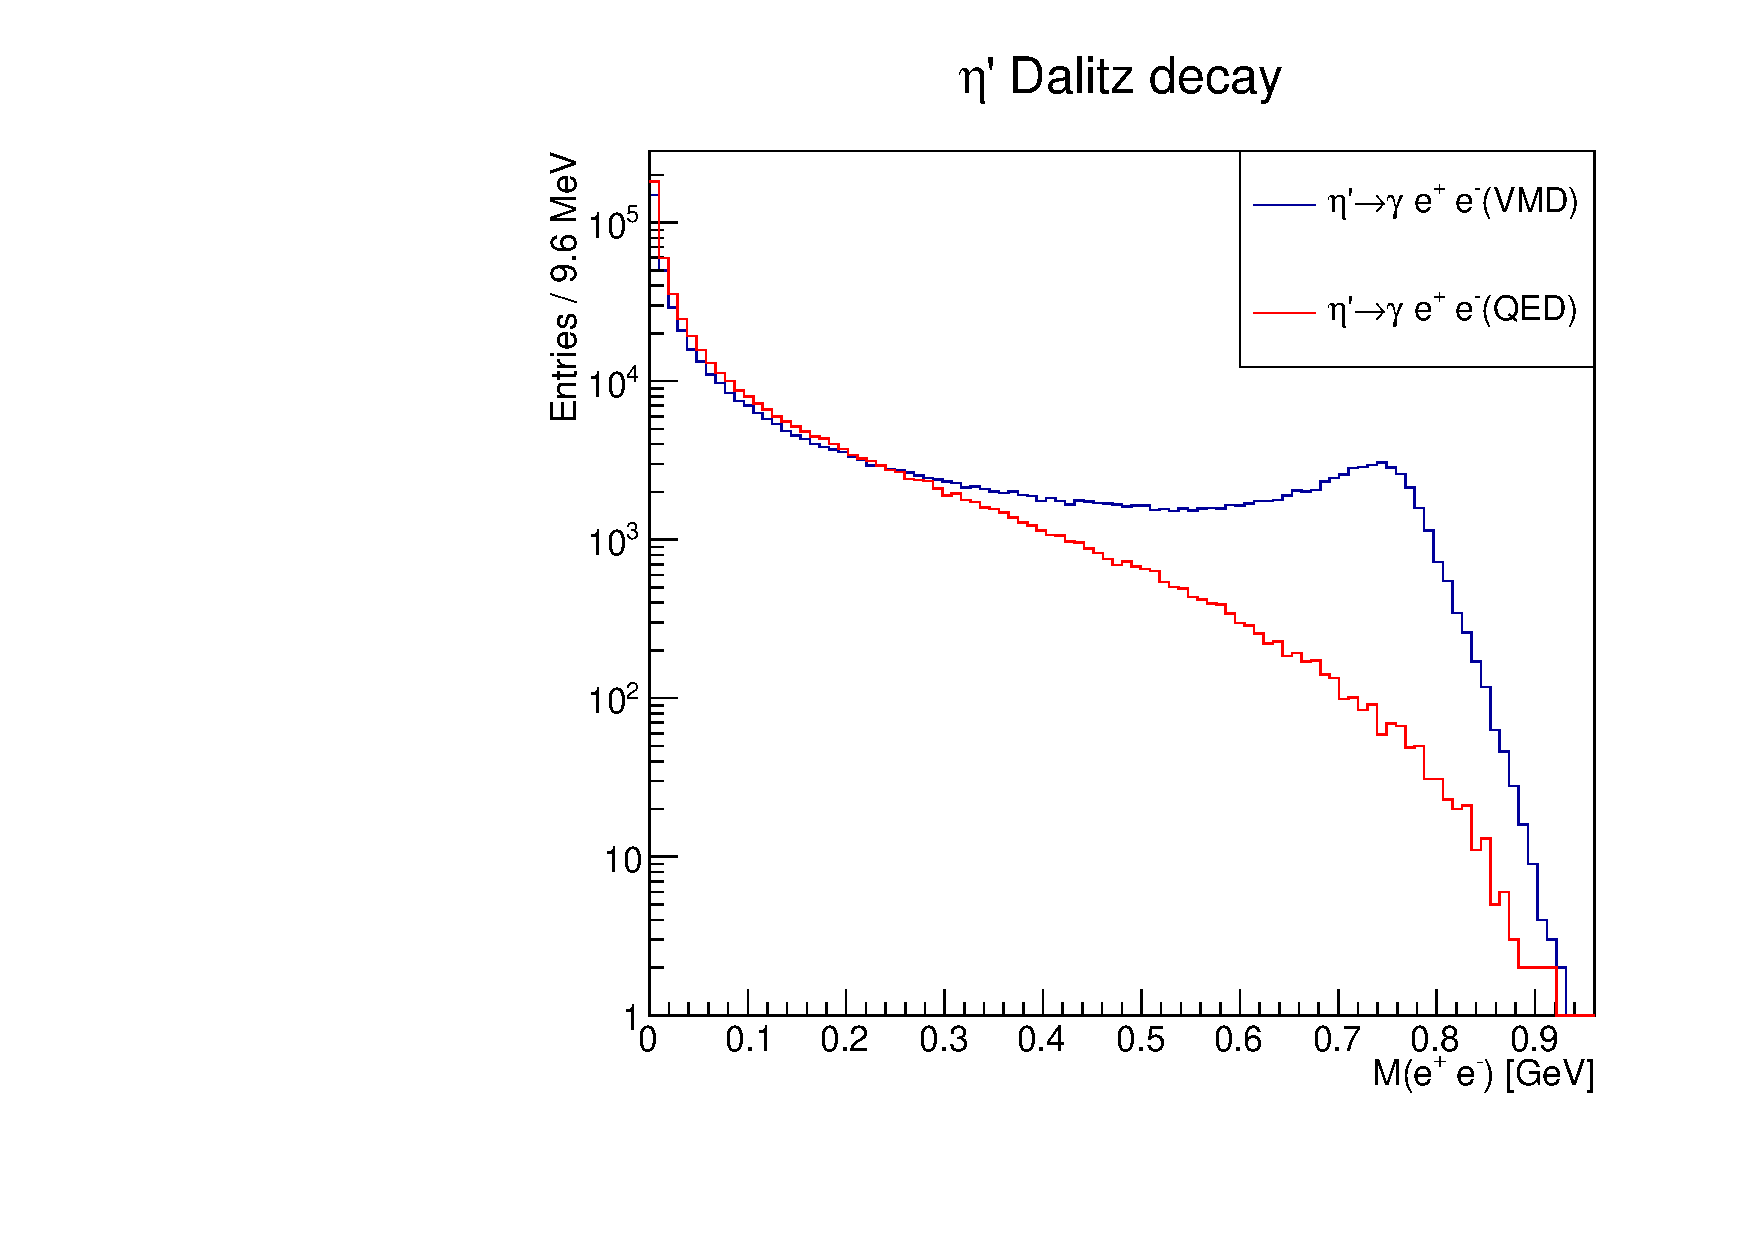
\includegraphics[width=0.8\columnwidth,height=1.0\qfigheight]{\grpath/decays/etaP_Dalitz_QED_FF_comparePlot.pdf}\label{fig:etap_dalitz_conpare}
 		\caption[Dalitz  for \etaTP \ and $\phi$]{\label{fig:dalitz_compare}Example of Dalitz spectra for \etaTP \ using only QED(red) and the deviation from QED using the VMD parameterization(blue) with 500K Dalitz events generated. }
 	\end{center}\end{figure}



% \begin{figure}[h!]\begin{center}
% 		\subfloat[$\etaP$ Dalitz spectra][]{ %Feynman diagram of $\etaP$ two photon decay
% 			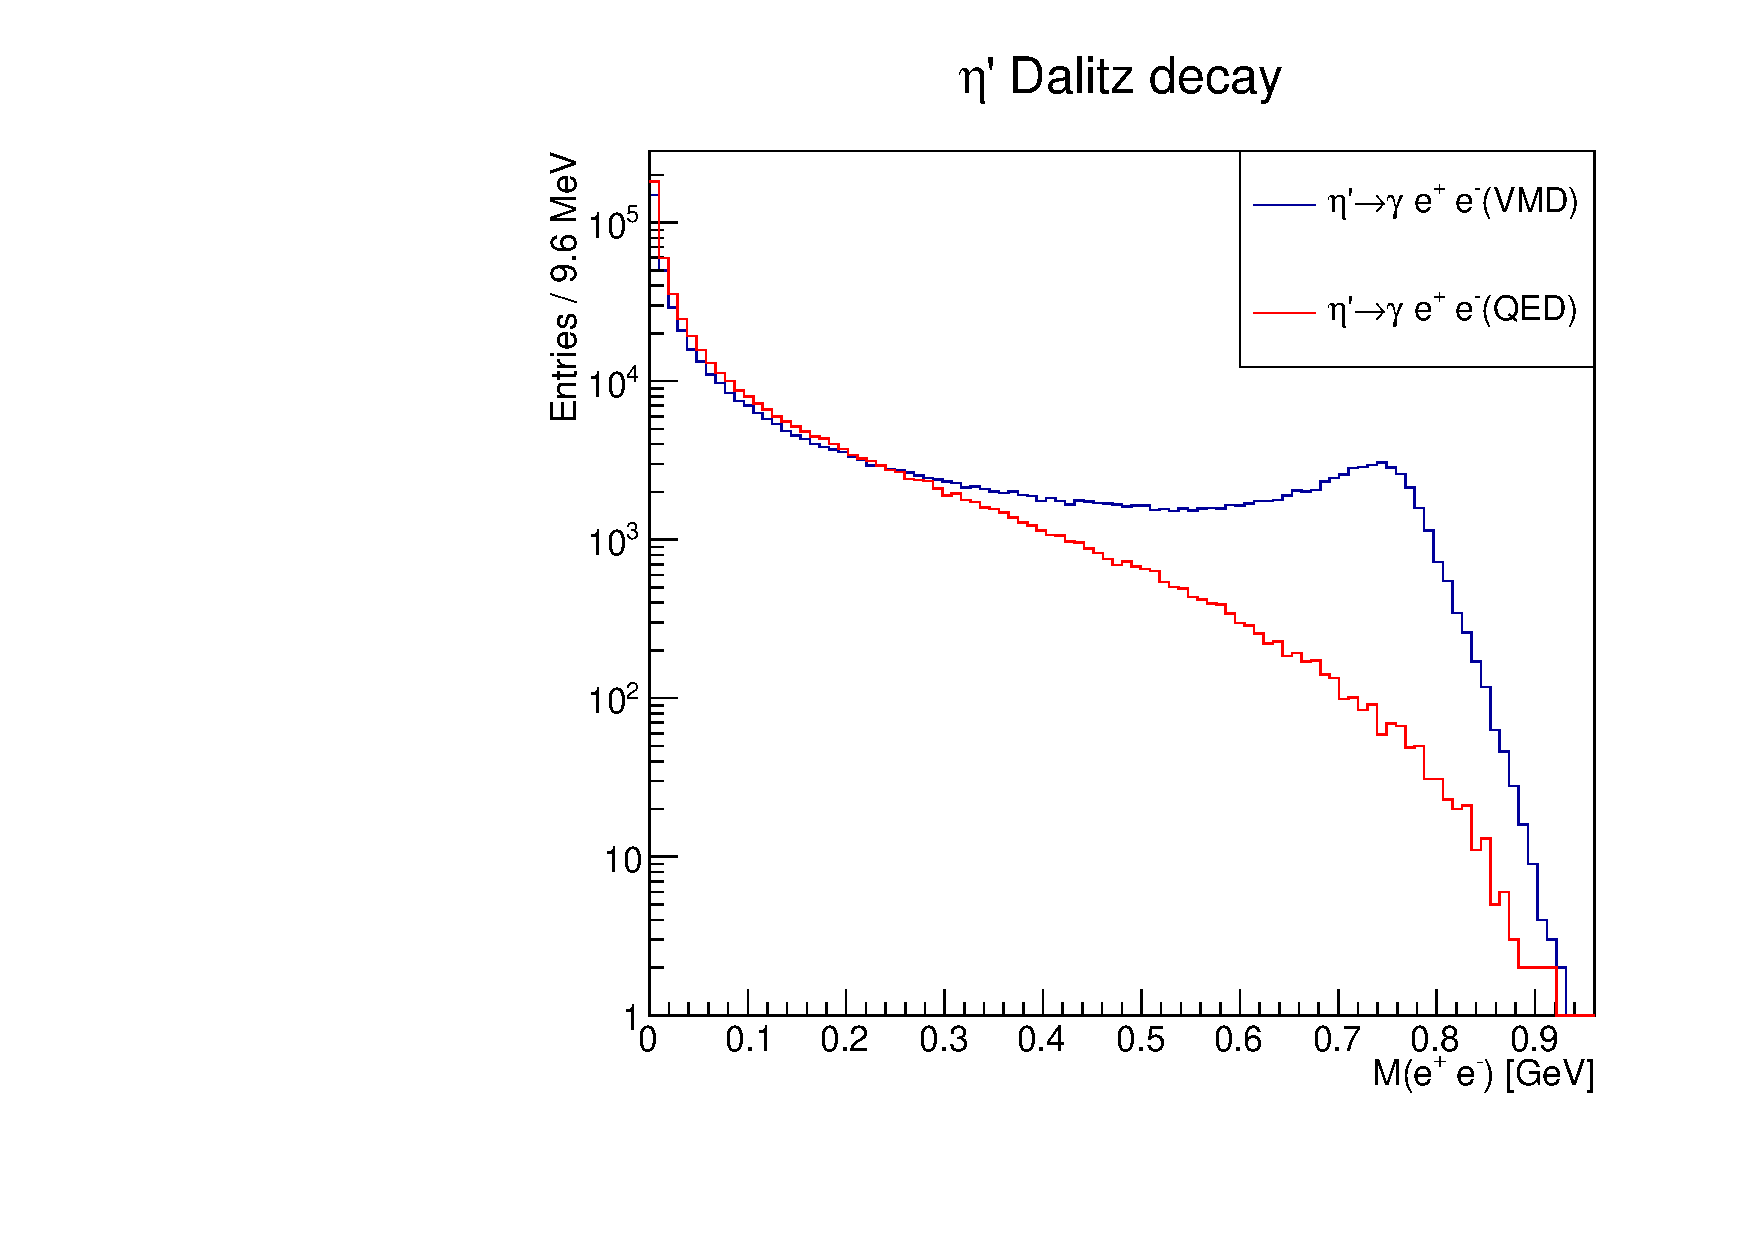
\includegraphics[width=0.8\columnwidth,height=1.0\qfigheight]{\grpath/decays/etaP_Dalitz_QED_FF_comparePlot.pdf}\label{fig:etap_dalitz_conpare}
% 		}
% 		%\quad 
% 		\\
% 		\subfloat[$\phi$ Dalitz  spectra][]{ %Feynman diagram of $\etaP$ Dalitz decay
% 			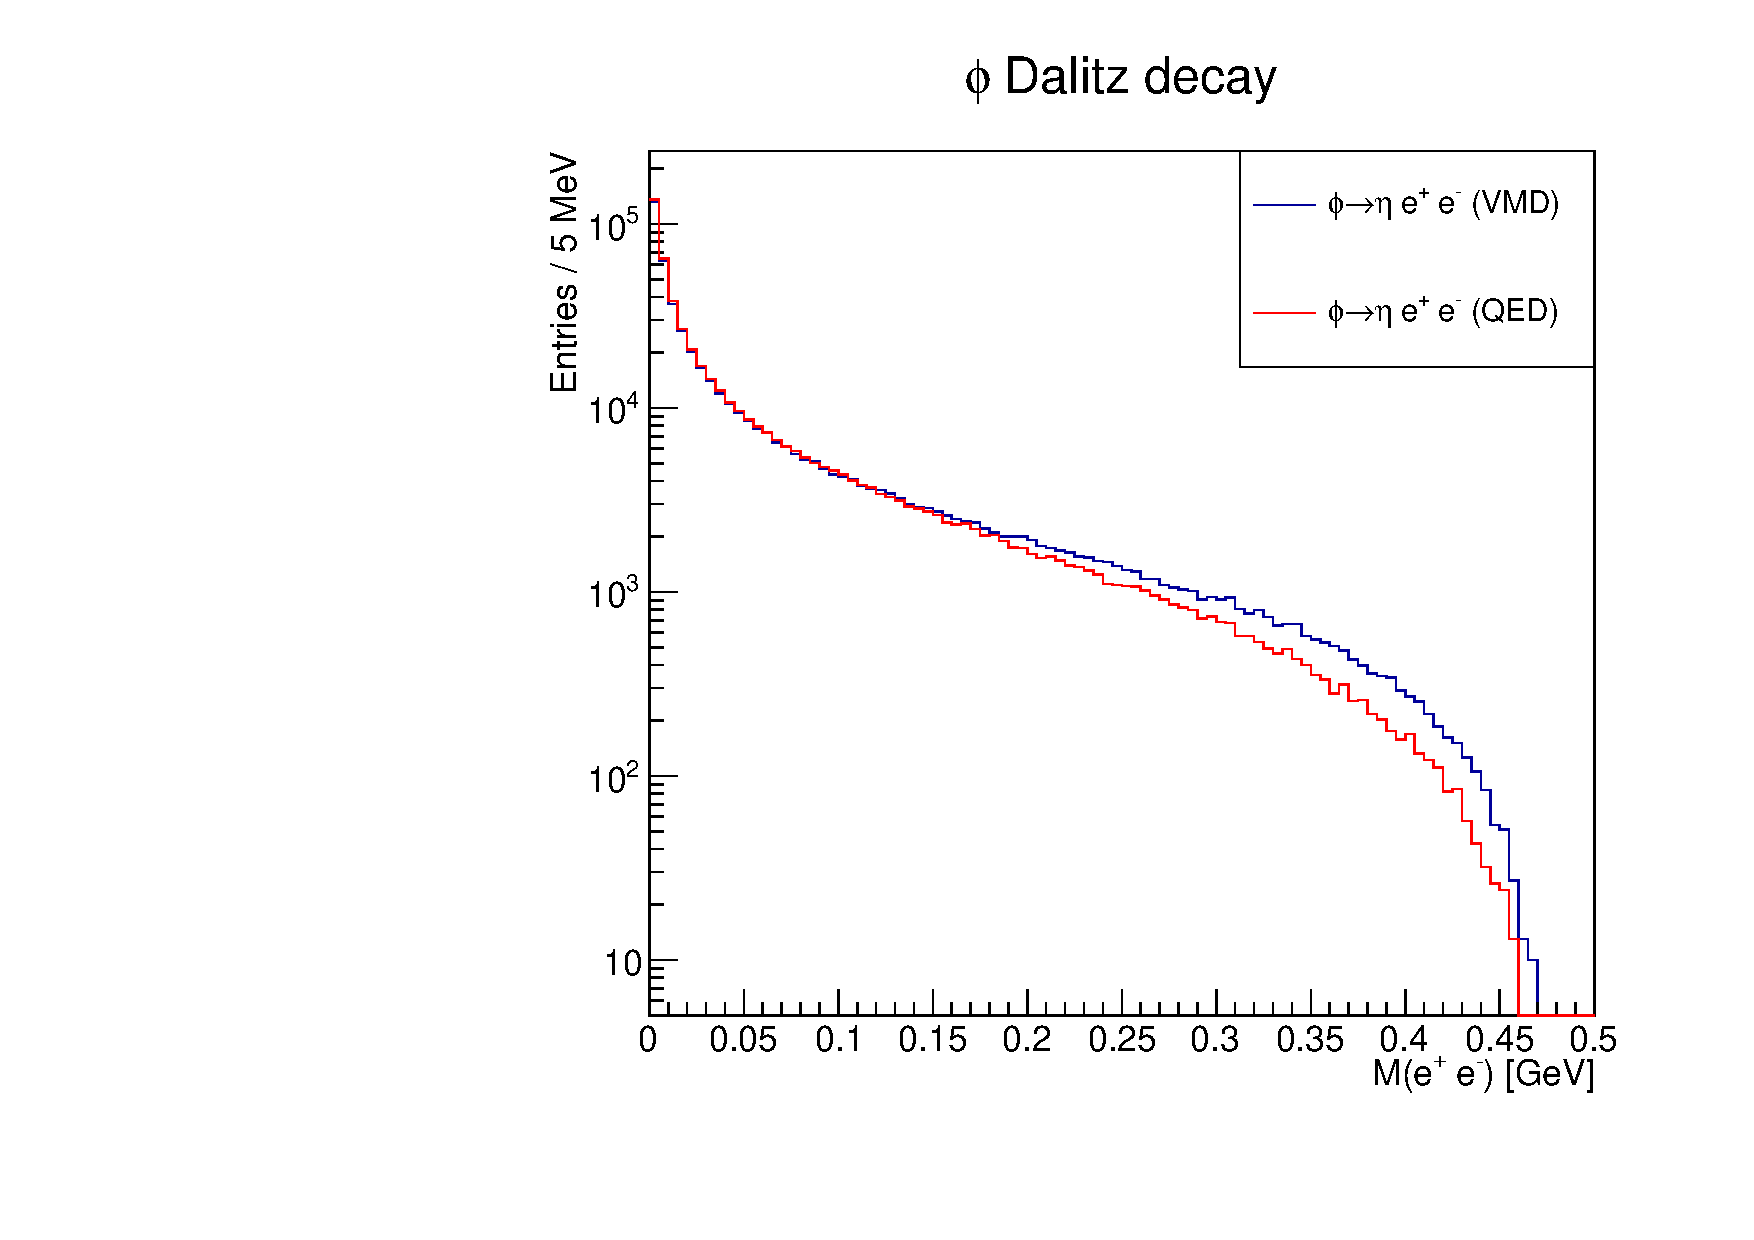
\includegraphics[width=0.8\columnwidth,height=1.0\qfigheight]{\grpath/decays/phi_Dalitz_QED_FF_comparePlot.pdf}\label{fig:phi_dalitz_compare}
% 		}
% 		\caption[Dalitz  for \etaTP \ and $\phi$]{\label{fig:dalitz_compare}Example of Dalitz spectra for \etaTP \ using only QED(red) and the deviation from QED using the VMD parameterization(blue) with 500K Dalitz events generated~\subref{fig:etap_dalitz_w_conversion}.  Example of Dalitz  spectra for $\phi$ using only QED(red) and the deviation from QED using the VMD parameterization(blue)  with 500K Dalitz events generated~\subref{fig:phi_dalitz_w_conversion}. }
% 	\end{center}\end{figure}
\FloatBarrier 	 
\subsection{Photon Conversion to \epemT Pairs}\label{sec:intro.conversion}
When a photon travels through matter at energies greater than 100~MeV, it can convert into an electron-positron pair. The process of pair production, $\gamma Z \rightarrow Ze^{+}e^{-}$, occurs when a photon with $E_0 > 2 m_e c^2$ converts into an electron and a positron. The cross section for this process can be written as;
\begin{equation}\label{pair_crosssection}
\sigma_{\gamma\rightarrow e^+e^-} =  \frac{A}{N_{A} \rho \lambda_\gamma}  \ ,\ \lambda_\gamma = \frac{9}{7}X_0
\end{equation}
where $\lambda$ is the interaction length, or mean free path, $\rho$ is the density of the material, $N_A$ is Avogadro's number and $A$ is the atomic mass of the material. The probability of pair production to occur is solely based on $X_{0}$, the radiation length of the medium and this probability can be expressed as;
\begin{equation}
\frac{dP}{dx} = \frac{1}{\lambda_\gamma}\exp(\frac{-x}{\lambda_\gamma}) \ .
\end{equation}
%
%
Using the ratio, $\frac{\Gamma_{\etaP \to e^+e^- \gamma}}{\Gamma_{\etaP \to \gamma \gamma}} = 2.13\cdot 10^{-2}$, that has been preliminary measured by CLAS, which is consistent with~\cite{BESIII}, the probability of pair production when a photon, from the $\etaP \to \gamma \gamma$ decay, traveling though 5~cm of liquid hydrogen, $\ell$H$_2$, is shown in Fig.~\ref{fig:conversion} as well as the number of $\etaP \to \gamma \gamma \rightarrow e^+e^- \gamma$ / $100 \etaP \rightarrow e^+e^- \gamma$. 
\begin{figure}[h!]\begin{center}
	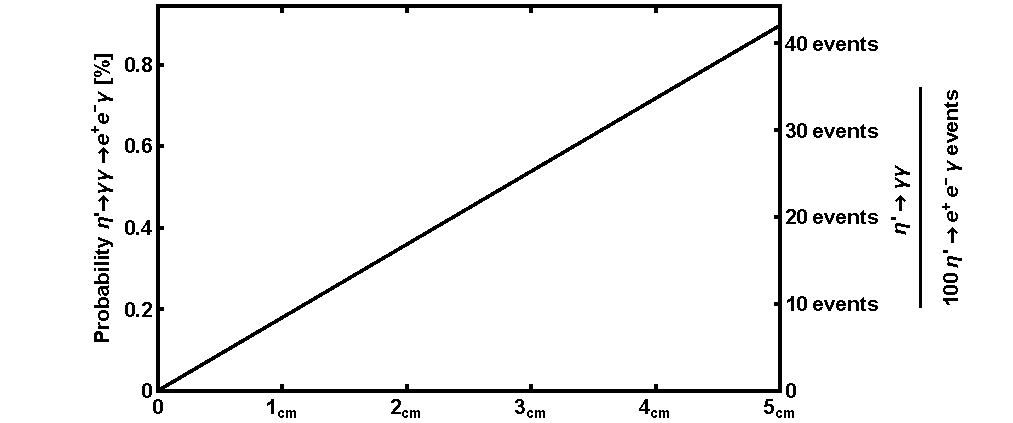
\includegraphics[width=\figwidth,height=\qfigheight]{\grpath/decays/cmplot.pdf}
	\caption[Probability of pair production, $\gamma \to$\epemT, as a function of distance in liquid hydrogen]{\label{fig:conversion}{(Left axis)Probability of pair production, $\gamma \to$\epemT; (Right axis) number of $\etaP \to \gamma \gamma \rightarrow e^+e^- \gamma$ / $100 \etaP \rightarrow e^+e^- \gamma$ as a function of distance in liquid hydrogen.}}
\end{center}\end{figure}
	Since CLAS12 has a vertex resolution of $\approx$1~mm the probability of pair production traveling through 10~mm is shown in Fig.~\ref{fig:conversionmm}. Therefore, a 1~mm cut on the primary vertex will yield a contamination of $\approx$ one externally converted \epemT from $\etaP \to \gamma \gamma \rightarrow e^+e^- \gamma$ per 100 Dalitz decays.
\begin{figure}[h!]\begin{center}
	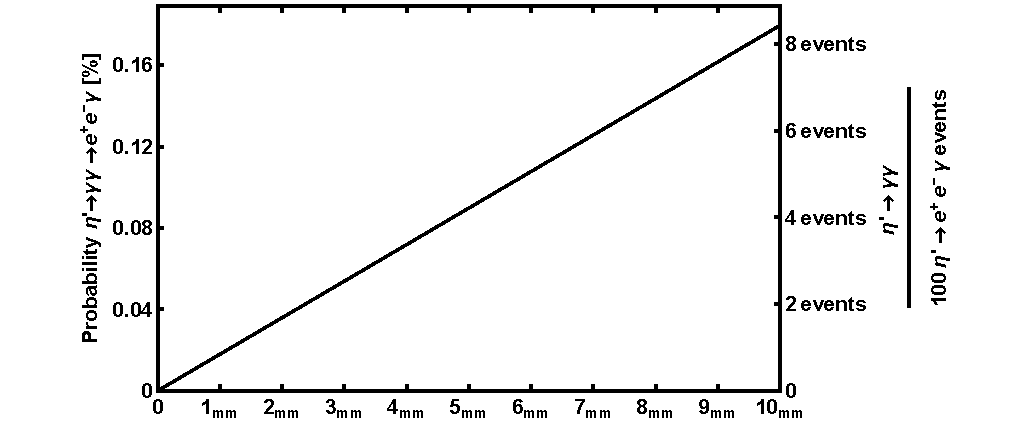
\includegraphics[width=\figwidth,height=\qfigheight]{\grpath/decays/mmplot.pdf}
	\caption[Probability of pair production, $\gamma \to$\epemT, as a function of distance in liquid hydrogen]{\label{fig:conversionmm}{(Left axis)Probability of pair production, $\gamma \to$\epemT; (Right axis) number of $\etaP \to \gamma \gamma \rightarrow e^+e^- \gamma$ / $100 \etaP \rightarrow e^+e^- \gamma$ as a function of distance in liquid hydrogen.}}
\end{center}\end{figure}
The external conversion process mimics the Dalitz decay  $\etaP \to e^+e^- \gamma$, described in Sec.~\ref{sec:dalitzdecay}. Since there are two photons with equal probability of conversion for $\etaP \to \gamma \gamma$, the total probabilities shown is for when either photon externally converts.
From multiple scattering effects the \epemT \ from a converted photon will obtain a mass distribution. Simulations of photons from \etaTP \ radiative decays traversing through 1~mm of $\ell H_2$  show that the \epemT can obtain a maximum mass of $\sim 0.14$~GeV.		
\begin{figure}[h!]\begin{center}
		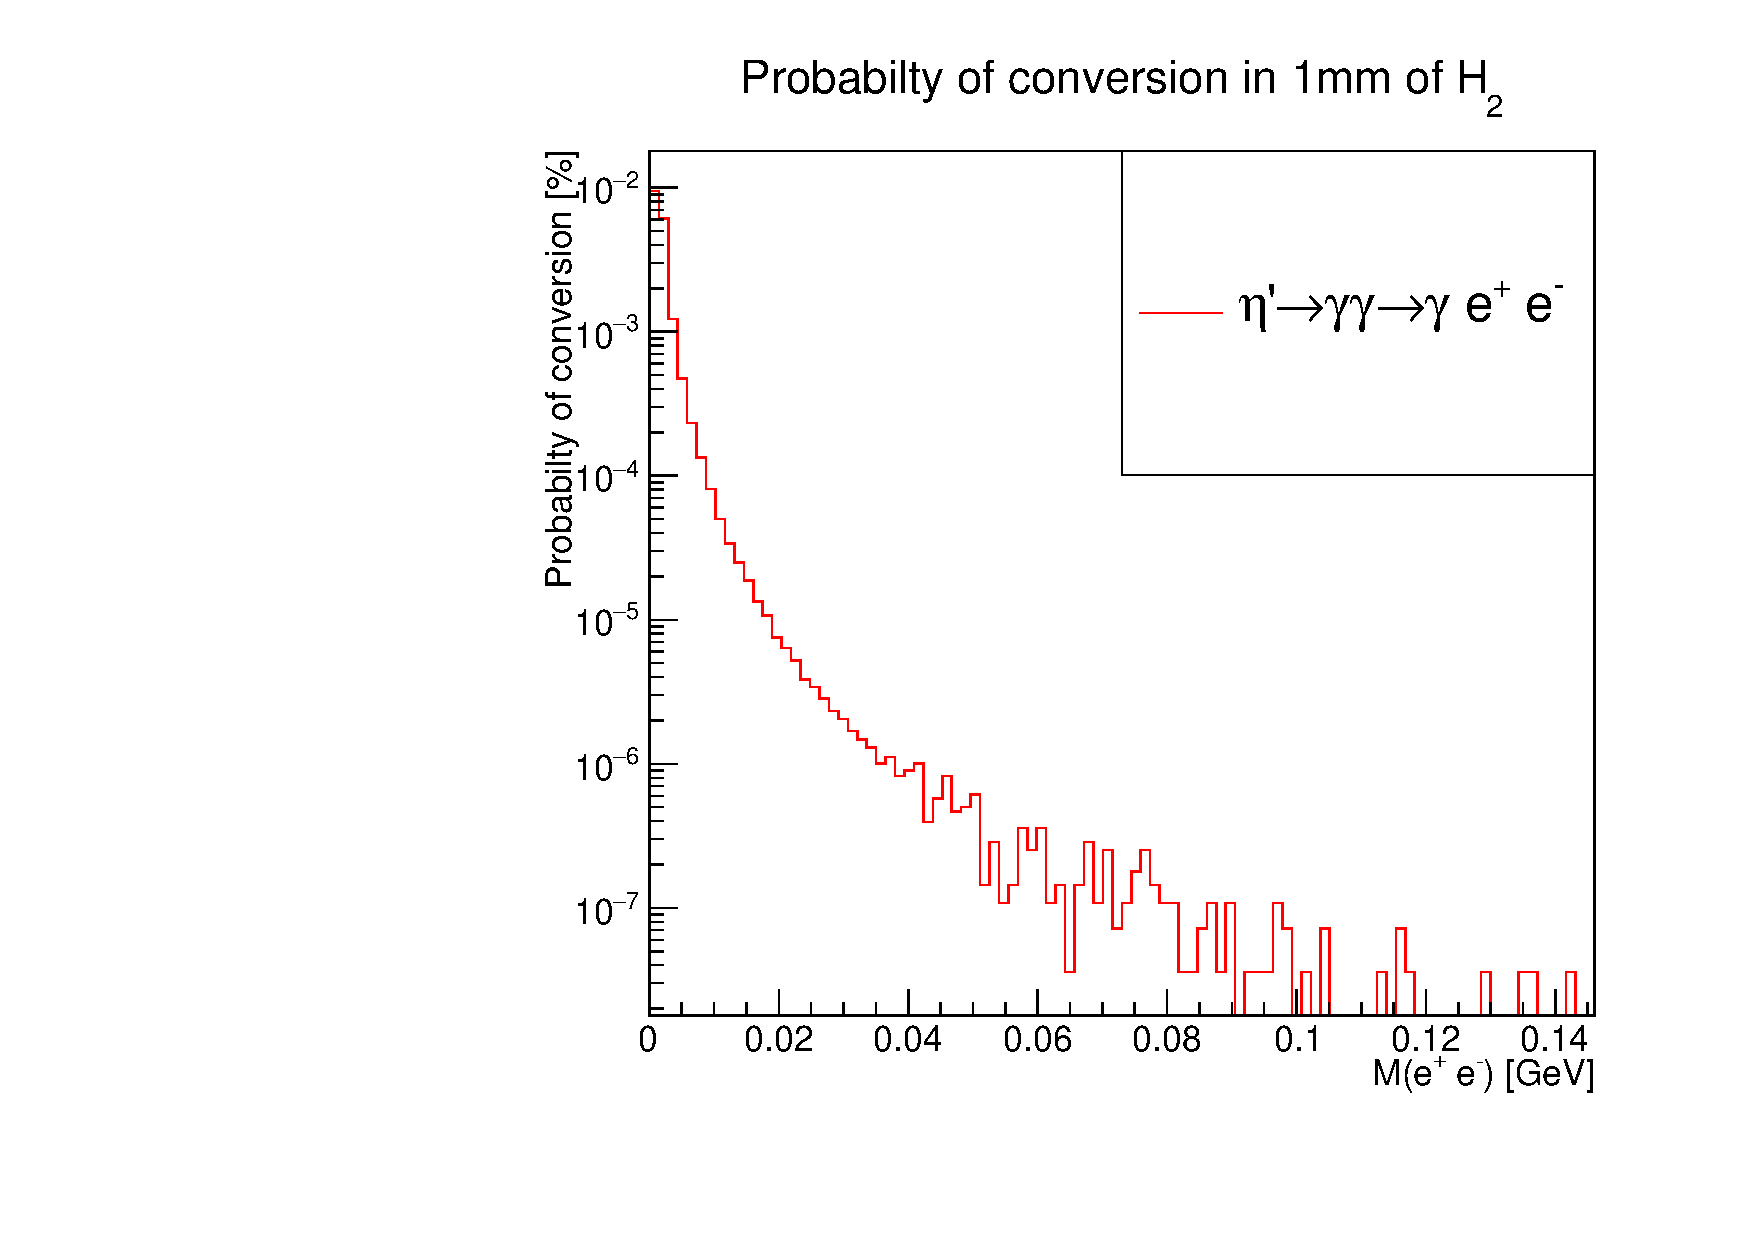
\includegraphics[width=\figwidth,height=1.2\qfigheight]{\grpath/decays/etaP_total_conversionPlot.pdf}
		\caption[Probability of pair production, $\gamma \to$\epemT, as a function of $M(\epem)$]{\label{fig:conversion_inM}{Probability of pair production in 1~mm of  $\ell H_2$ for $\etaP \to \gamma \gamma $ vs. $M(\epem)$.}}
\end{center}\end{figure}
\FloatBarrier
 \subsection{Summary}
 The $\gamma \gamma$ decay and the $\gamma^\star \gamma$ decay have different branching ratios. This difference is attributed to the factor of $\alpha$ along with a $q^2$ dependence calculated in the Dalitz decay. However, due to the probability of a photon converting into an electron-positron pair in $\ell$H$_2$, the total amount of \epemT pairs produced via photon conversion can contaminate the measurement of the form factor. The CLAS detector will have vertex resolution of $\sim$1~mm, therefore the amount of contamination of externally converted pairs will be minimized by the vertex position of the \epemT pair. An example of the total contamination, in the Dalitz spectrum, from external conversion within 1~mm of the primary vertex can be seen in Fig.~\ref{fig:dalitz_w_conversion}.
 \begin{figure}[h!]\begin{center}
 			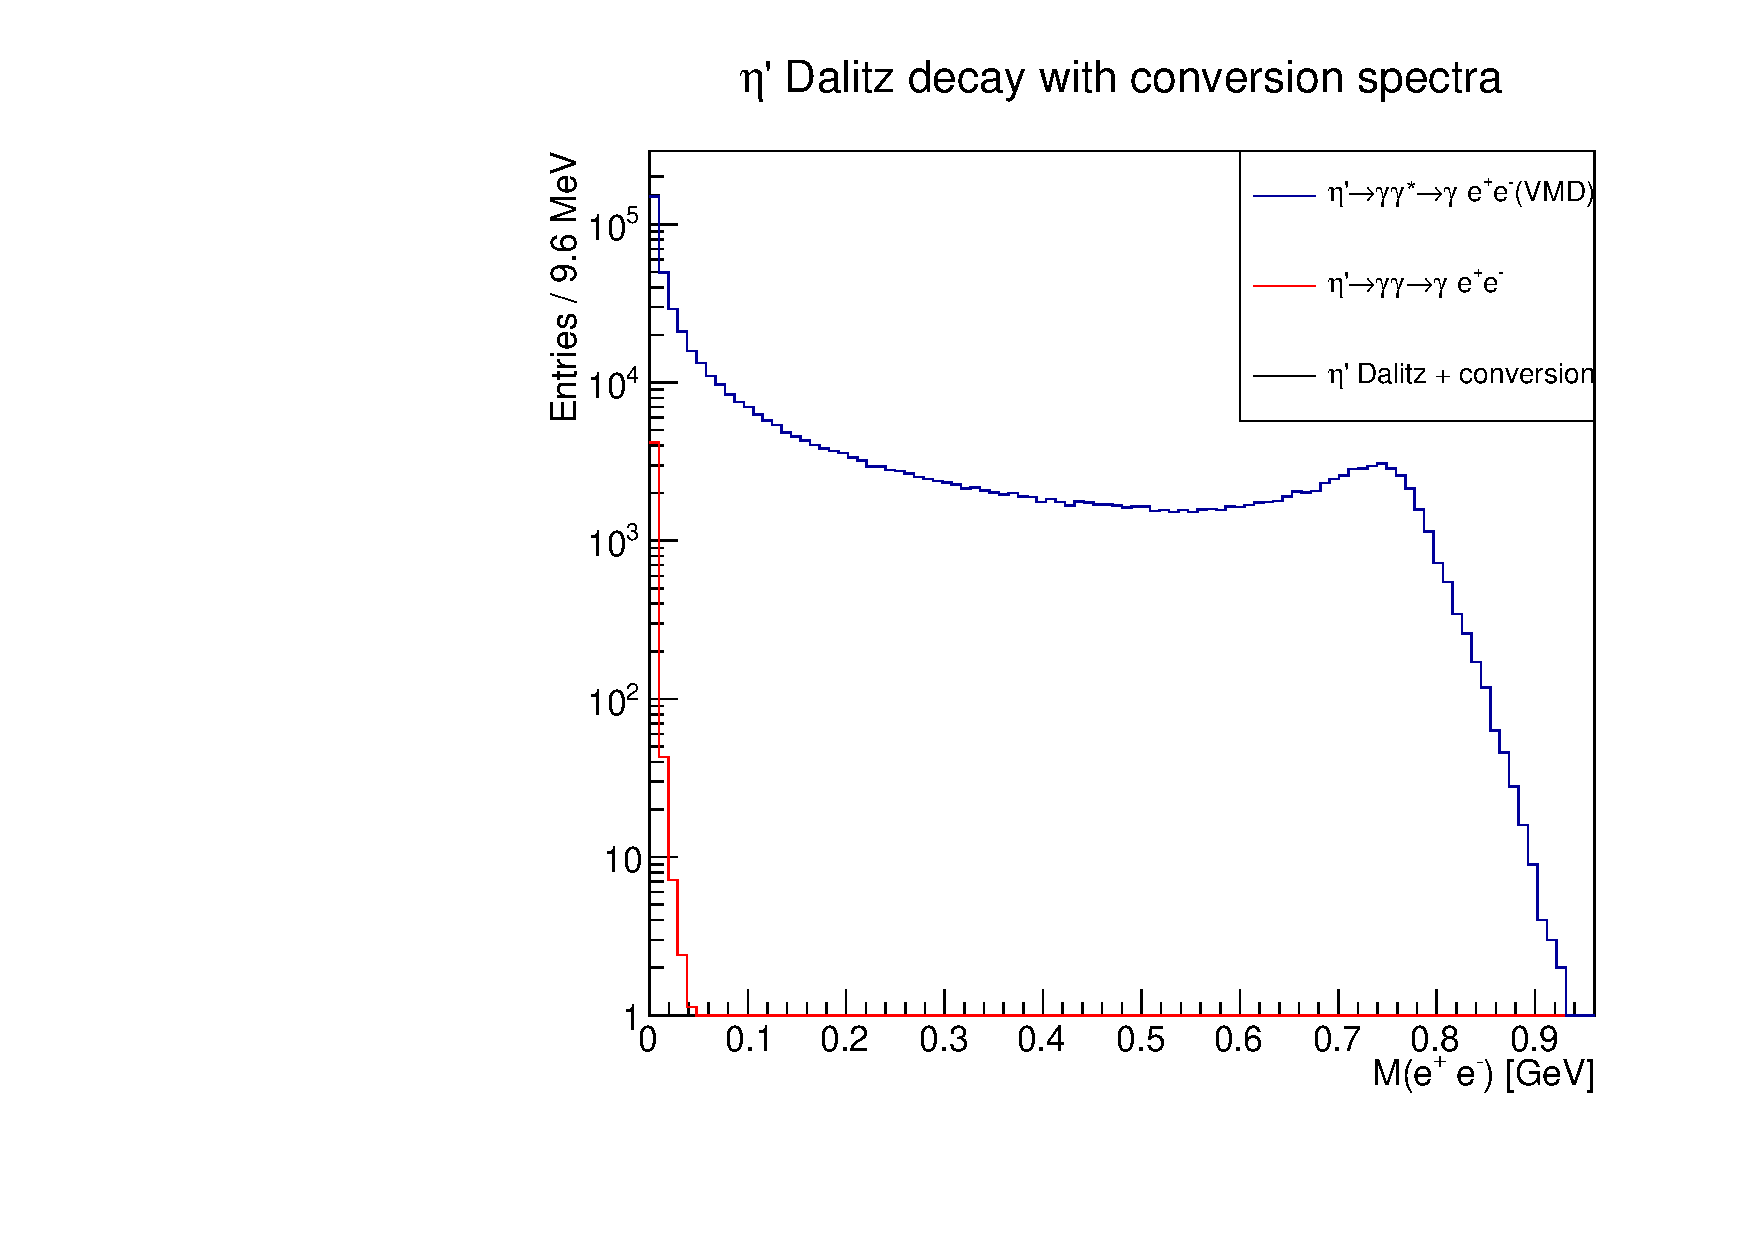
\includegraphics[width=0.8\columnwidth,height=1.0\qfigheight]{\grpath/decays/etaP_Dalitz_decay_with_conversion_spectra.pdf}
\caption[Dalitz and conversion spectra for \etaTP \ and $\phi$]{\label{fig:dalitz_w_conversion}Example of Dalitz and conversion spectra for \etaTP \ with 500K Dalitz events generated and $\sim 2.35 \cdot 10^7$ $\etaP \to \gamma \gamma$ generated.}
\end{center}\end{figure}
\FloatBarrier
  
  
  